In this section, we empirically evaluate STOIC's performance on image processing tasks. We implement the application as a serverless function for STOIC to schedule and execute.

In each experiment, STOIC determines which resource to use for function execution (among a small set of feasible choices). We then run the function on \textit{all} resources and compare the choice made by STOIC to the best (shortest duration) execution across all possible choices.

\subsection{Experimental Setup}

The image processing application that we use as a benchmark classifies animal images from a wildlife monitoring system.
%called ``Where's The Bear"
%(WTB)~\cite{ref:wtb}. ``Where's The Bear" is an end-to-end distributed data
%acquisition and analytics system that automatically analyzes camera trap
%images collected by cameras sited at the Sedgwick Natural
%Reserve~\cite{ref:sedgwick} in Santa Barbara County, California. The WTB
Our deployment includes an edge cloud located near the cameras that acquires the data from the cameras. The edge cloud is connected via a slow (microwave) link to a private cloud located at a research facility located approximately 50 miles from the site. In this work, we explore using the Nautilus distributed GPU cloud~\cite{ref:nautilus} as the public cloud, in conjuction with the edge cloud to optimize image classification on a convolutional neural network (CNN)~\cite{ref:cnn} implemented by Tensorflow and Scikit-learn~\cite{ref:scikit}. 

In total, there are five classes that we consider: Bird, Fox, Rodent, Human and Empty. Since class size is unbalanced due to the frequency of animal occurrences, we up-sample minority classes (e.g. fox) using the Keras ImageDataGenerator~\cite{ref:keras}. Doing so ensures that the classification model is not biased. We resize every image in the image dataset to $1920 \times 1080$, and for each class, the dataset contains 251 images used to train the CNN model. Once model training is complete, the application stores this model in hdf5 format in object storage at both edge cloud and Nautilus.

As described previously, STOIC moves images from the wildlife refuge to the public cloud in batches. To better harness the multiple GPU runtime of the public cloud, the application spawns a process (wor\-ker) for each GPU and adds all images in a batch to a shared asynchronous queue. Upon the execution, workers remove images (one at a time) from the shared queue until it is exhausted. This mechanism ensures multiple GPU runtimes evenly divide the workloads among GPUs and achieve quasi-linear acceleration at the application level, where the perfect linear speed-up is unattainable because of model loading and memory transfer overhead~\cite{ref:multi_gpu}. 


\iffalse
\subsection{Deployment Options}

We explore four different deployment options on STOIC: 
\begin{itemize}
\item a node of the edge cloud (Edge), 
\item on the controlling CPU (an x86 processor) that Nautilus uses to move
data in and out of one or more GPUs (CPU),
\item on one GPU in Nautilus (GPU1),
\item on two GPUs in Nautilus (GPU2).
\end{itemize}
On the edge cloud, the application begins immediately when a camera delivers an image batch.  To use Nautilus, however, the image batch must first traverse the network from the edge cloud to Nautilus (thereby incurring an additional transfer time) and then Nautilus must schedule a ``pod'' (containing either one or two GPU in this study) before the Nautilus CPU or any GPU can begin running.  We define the time that Nautilus requires for pod scheduling as ``deployment time.''~\footnote{Note that Nautilus currently allows non-priviledged users to request up to 8 GPUs, but the deployment times for requests of greater than 2 are usually large as to make them superfluous. That is, a GPU request for more than two GPUs is rarely, if ever successfully, satisfied in the shortest possible time.} Finally, the run time is the time required by a resource (Edge, CPU, GPU1, and GPU2) to complete the CNN training.  

We do not explore the possibility of overlapping transfer time, deployment time, and run time and we do not model the time required to return the trained model to the edge cloud. Thus the total response time is the sum of the transfer time, the deployment time, and the run time for an image batch. On the edge, the transfer times and deployment times are zero.
\fi



\begin{figure*}[t] \centering 
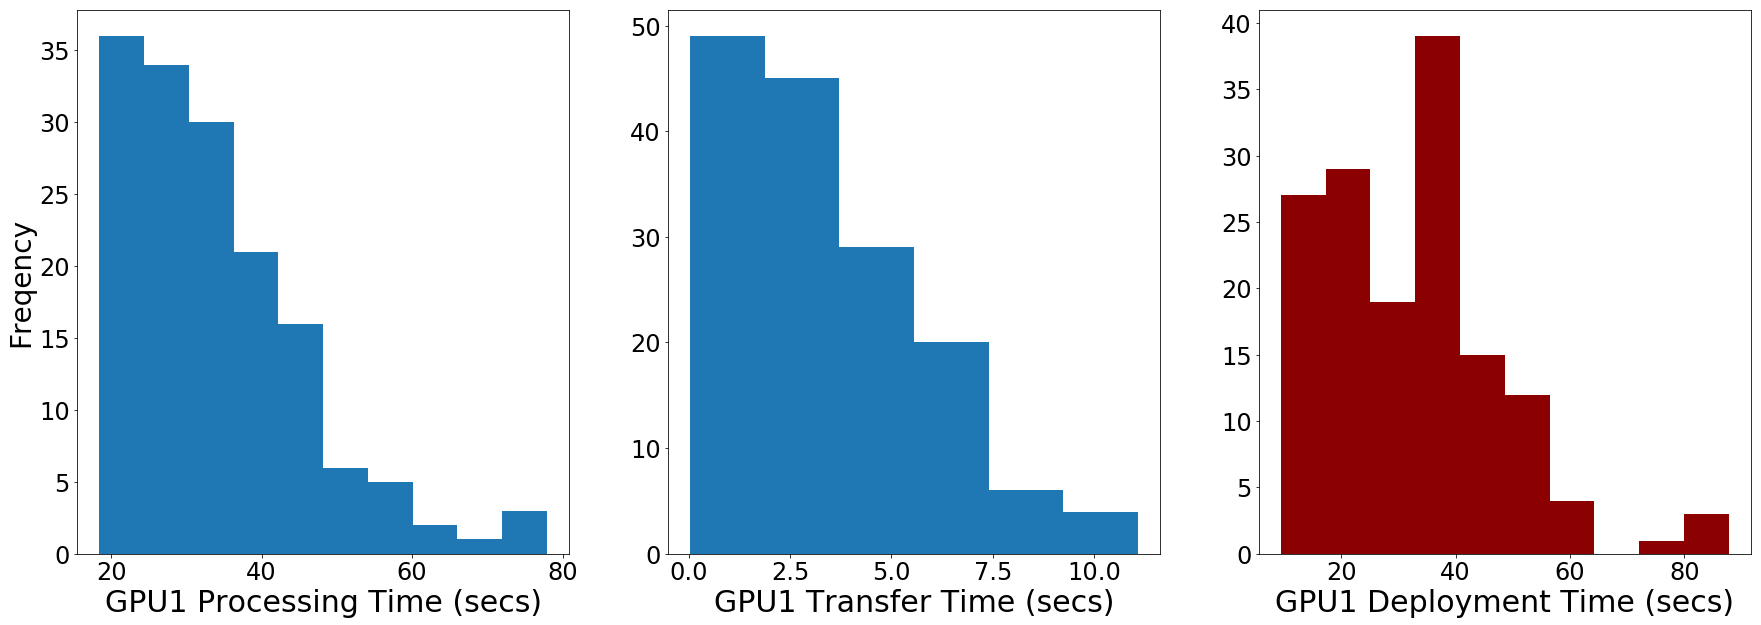
\includegraphics[scale=0.24]{figures/gpu1_latency.png}
\caption{The distribution of three components in total response time~($T_s$) of 150 executions on GPU1 runtime: Processing time ($T_p$), Deployment time ($T_d$) and Transfer time ($T_t$). The x-axis represents the time range, while the y-axis is the frequency of executions. The deployment time, which is depicted in the red histogram, is volatile and error-prone to prediction.
\label{fig:breakdown}}
\end{figure*}

To drive this experiment, we use the workload generator described in Section~\ref{sec:workloadgen} to facilitate faster-than-real time evaluation of STOIC. The generator uses a image series and their inter-arrival patterns from a camera trap image corpus ranging from 2013 to 2017. Figure~\ref{fig:breakdown} shows example histograms for processing time, transfer time, and deployment time on Nautilus for GPU1 runtime using 150 batches drawn from the workload generator. On the x-axis, we show the elapsed time for processing time, transfer time, and deployment time respectively. Note that processing time and transfer time are relatively stable compared to deployment time. 

\subsection{Selector Evaluation}

We first evaluate STOIC selector mode for a 24-hour time period consisting of 162 image batches, the sizes of which are drawn randomly from the workload generator. Each batch is executed on the edge cloud, on the Nautilus CPU, on one Nautilus GPU and on two Nautilus GPUs. Over the test period, the STOIC Selector chooses the fastest (lowest total response time) from among these four options $149$ times out of the $162$ runs or $92\%$ of the time. That is, STOIC correctly identifies the fastest option with a success rate of $92\%$.

Further, the optimal selection (i.e. an oracle selection that is $100\%$ correct) would have resulted in an aggregate total latency of $10022$ seconds and the worst case aggregate latency as $35940$ seconds compared to a STOIC aggregate latency of $10770$ seconds.  Thus STOIC achieves an aggregate latency that is $7.4\%$ slower than optimal, but $70\%$ ($3.33$) times faster than the worst case.

%Table~\ref{tab:selector} summarizes these results. In the
%table, we report the success rate, the percentage of optimal, and the
%percentage of worst case aggregate response times achieved by STOIC. 

%\begin{table}[t] 
%\begin{centering}
%\captionsetup{justification=centering}
%\scriptsize
\resizebox{\columnwidth}{!}{
\begin{tabular}{|c|c|c|} 
\hline
\textbf{Success Rate} & \textbf{versus Optimal} & \textbf{versus Worst Case}\\
\hline
$92\%$ & $105\%$ & $30\%$ \\
\hline
\end{tabular}
}

%\end{centering}
%\caption{
%STOIC Selector results. The success rate is the percentage of correct decisions
%(out of 162 trials) made by STOIC.  ``Optimal'' shows the percentage of the
%optimal selection aggregate response time and ``Worst Case'' shows the percentage of the worst case 
%selection aggregate response time made by STOIC.}
%\label{tab:selector}
%\end{table}

We further analyze the data points where STOIC made erroneous selections and found two sources of error. First, the most error occurs around two batch sizes where the total response times of runtime have approximately same latency. To be specific, the edge and GPU runtimes cross over at 35 image batch size, and 90 image batch size for the GPU1 and GPU2 runtimes. At these cross-points, the close predictions of latency lead to incorrect selection. Second, the deployment times for GPU runtime are volatile and error-prone to prediction. As a representative instance, Figure~\ref{fig:breakdown} demonstrates the distribution of processing time ($T_p$), transfer time ($T_t$) and deployment time ($T_d$) of GPU1 runtime. We observe geometric distribution from the histogram of processing time and transfer time, whereas deployment time varies irregularly with many outliers. These two phenomenons lead to mistaken selections in the experiment.

\subsection{Duplicator Evaluation}

Note that the edge cloud node is not a shared resource -- it is dedicated to the application. It is implemented using inexpensive hardware that is connected to standard 120 VAC power (in a closet in a management building located at the refuge).
%at Sedgwick).  
As a result, it is possible to use the edge cloud for \textit{every} batch even when it is not the fastest.  

Put another way, there is no cost to running the edge cloud speculatively while data is transferring to Nautilus and the application waits for Nautilus to deploy pods for the CPU and GPUx runtimes. If STOIC (using Selector) predicts that Nautilus will be faster, and STOIC is correct, the work on the edge cloud is ``duplicate work'' which is unnecessary. However because of the deployment variability, it may be that the edge cloud speculative execution finishes ahead of that runtime scheduled to Nautilus.

However, unlike the edge cloud node, Nautilus is a shared resource.  Thus we do not wish to ``waste'' execution time on Nautilus unnecessarily. Thus, in this setting, the cost of duplicate work on the edge is minimal compared to the cost of potentially duplicate work on Nautilus. If this were not true, we would simply launch the job both at the edge and on Nautilus and use whichever finished first.

Thus we explore a second scheduling strategy that attempts to minimize total response time in light of the following assumptions:
\begin{itemize}
\item Duplicating unneeded work on the edge carries no penalty.
\item Duplicating unneeded work in Nautilus is expensive.
\item The STOIC predictions (initial and after transfer and deployment) will be used to
choose the resource that yields the fastest response time while using the
Nautilus resources parsimoniously.
\end{itemize}
We call the STOIC scheduler that attempts to minimize response times under these assumptions -- the Duplicator.

Further, we noticed that the Naultilus CPU is seldom a good choice in practice. The application must ``pay'' for the transfer and incur the deployment time variability to acquire a CPU that is almost equivalent to the edge node CPU.  Thus, in the ``real world'' version of the STOIC scheduler for the application, we use the Duplicator with Nautilus GPUs only.

The scheduling algorithm starts the task on the edge cloud node and also begins the transfer to Nautilus. It then waits for the Nautilus deployment time and, when the pod is fully deployed, it predicts whether to use the freshly acquired GPU or GPUs (i.e. to ``switch'' to the GPU(s)) or to abandon the request and to complete the job on the edge.  To do so, STOIC must predict the \textit{remaining} edge time at the moment the GPU pod is deployed, and compare this remaining time to the predicted GPU processing time.  

The Duplicator prediction is \textit{conditional} upon the amount of time that has elapsed during transfer and deployment to Nautilus. If STOIC predicts that the GPU pod will start and complete their processing before the edge completes what remains of the job, it allows the Nautilus and edge cloud executions to execute concurrently. If the Nautilus job completes first, the edge cloud execution is terminated.  Otherwise, if the edge cloud execution finishes first (i.e. the prediction was incorrect) then the Nautilus job is terminated (and the time between the start of the Nautilus job and the end of the cloud job is ``wasted'' Nautilus time).

Alternatively, when STOIC predicts that the edge cloud will finish first, it returns the GPU resources to Nautilus and run only the edge cloud job. If the Nautilus job would have completed first (i.e. the conditional prediction in favor of the edge is incorrect) then the time between when the Nautilus job would have finished and the time that the edge cloud job completes is additional delay (compared to having made a correct prediction).

Thus, choosing incorrectly (i.e. a failure) occurs when the actual completion time exceeds the time of the runtime corresponding to the minimum prediction (in either edge or GPU case) made by STOIC. That is, a ``failure'' for the Duplicator occurs when STOIC makes a conditional choice (i.e. continue on edge or to include Nautilus) and the choice results in a longer \textit{actual} response time than the one not chosen. Table~\ref{tab:comparison} shows the performance of the Duplicator using the edge and one GPU and, separately, the edge and two GPUs from Nautilus. 

%We duplicate the results for the Selector from Table~\ref{tab:selector} for comparison purposes.

\begin{table*}[t] 
\centering
\captionsetup{justification=centering}
\scriptsize
\resizebox{\columnwidth}{!}{
\begin{tabular}{|c|c|c|c|} 
\hline
& \textbf{Success Rate} & \textbf{versus Optimal}  & \textbf{versus Worst Case}\\
\hline
Selector  & $85\%$ & $108\%$ & $45\%$\\
\hline
Duplicator Edge vs GPU1 & $97\%$ & $102\%$ & $45\%$\\
\hline
Duplicator Edge vs GPU2 & \textbf{$95\%$} & \textbf{$101\%$} & \textbf{$45\%$} \\
\hline
\end{tabular}
}

\caption{
The comparison of Selector and Duplicators}
\label{tab:comparison}
\end{table*}

These results are both expected and surprising. As expected, restricting the choice to edge and a single Nautilus request and using a conditional prediction at deployment time (as opposed to a ranking at the beginning) as a success criterion improves the success rate dramatically. We do not claim that Duplicator is better than Selector in terms of success rate. Instead, Duplicator enables a more dependable scheduling strategy for the classification application based on conditional predictions rather than resource ranking. Surprisingly, however, requesting 2 GPUs improves both success rate and aggregate response time relative to choosing one.

This result surprised us for two reasons. First, because there was greater deployment variance and a larger mean deployment time for two GPUs, we expect that the edge (which is more predictable) would generate a greater success rate, but a larger aggregate response time. Put another way, we expected that STOIC would make safer predictions favoring the edge in the GPU2 case, but the cost of this safety would be greater aggregate response time. Empirically, however, we observe that STOIC ``risks'' predicting the GPU2 deployment more frequently, but that it amortizes this risk effectively because the two GPU execution is faster.

Note that the cost is not large. In practice, the application
%WTB project 
will use the one GPU case to get a better success rate at the cost of $2\%$ in aggregate response time.  However, it is interesting that STOIC is able to make this risk-reward trade-off explicit. Note also that the worst case is unchanged. This result indicates that there are unusually bad response time, but that \textit{all} STOIC scheduling methods can mitigate them to approximately the same degree.

We conclude our analysis with a quantification of the savings and unnecessary loss of Nautilus time that STOIC Duplicator is able to achieve. Table~\ref{tab:savings} shows the savings and loss of Nautilus time that are realized by the Duplicator heuristic.

%
%error Duplicator makes
%with respect to the STOIC conditional predictions.
%We define Mean Deadline Error (MDE) as the mean over prediction (in seconds)
%made by STOIC in the case the actual total response time exceeds the predicted
%total response time.
%$MDE = \frac{1}{n}\sum(L_g - L_e)
%\,|\ if \ L_g > L_e \ \& \ R_s = GPUx $, where $L_g$ is the latency of GPU
%runtime, $L_e$ is the latency of edge cloud, $R_s$ is the actual runtime by
%STOIC. 
%We define the ``Mean Overprediction Error'' (MOE) as the average
%overprediction that Duplicator makes when it fails to choose the fastest
%option.
%Based on the experiment data, the MOE for edge and one Nautilus GPU is $27$ seconds 
%and for edge and two Nautilus GPUs it is $44$ seconds.
%Thus, when Duplicator fails to choose correctly, the average ``miss''
%is under a minute.
%

\begin{table}[t] 
\centering
\scriptsize
\resizebox{\columnwidth}{!}{
\begin{tabular}{|c|c|} 
\hline
\textbf{STOIC Choice} & \textbf{Nautilus Savings (+) or Loss (-)}\\
\hline
edge & $+1393$s\\
\hline
1 gpu & $-440$s\\
\hline
2 gpus & $-257$s\\
\hline
\end{tabular}
}

\caption{
Nautilus savings (positive values) and loss (negative values) for STOIC Duplicator. Savings are the time returned to Nautilus due to edge execution. Loss is the ``wasted'' time on Nautilus when the GPU runtimes are terminated because of faster edge execution. All units are in seconds. In the GPU2 case, the time is for both GPUs.}
\label{tab:savings}
\end{table}

Recall that the total optimal time (the time associated with the minimum execution of each batch) is $10022$ seconds. The positive values in the table indicate the total time returned to Nautilus (that would have otherwise been used) by selecting the edge for execution.  Note that these savings correspond to the results shown in Table~\ref{tab:comparison} for the Duplicator. That is, they are the savings that STOIC was able to achieve while implementing a schedule within either $1\%$ or $2\%$ of optimal.  The loss (negative values) shows the amount of Nautilus time that was used unnecessarily. That is, when STOIC Duplicator chose conditionally to use the GPU or GPUs and the edge finishes first, the elapsed time on Nautilus is unnecessarily ``lost.'' Clearly from the table, Duplicator saves more Nautilus time than it loses. Thus, we infer that STOIC in duplicator mode optimizes the time to solution (Table~\ref{tab:comparison}) while utilizing the expensive Nautilus resource efficiently (Table~\ref{tab:savings}) by using the edge cloud node speculatively.  


% (47.43\% to the
%mean gpu2 runtime latency). This result implies that the unstable deployment
%time of GPU runtimes significantly affects the accuracy of prediction made by
%STOIC. 

%To address the above issue, we reconfigure STOIC into the duplicator mode
%demonstrated in Figure~\ref{fig:duplicator}. Based on the historical data,
%the selector makes prediction and only execute workload at the runtime with
%least total latency, whereas the duplicator runs workload on edge cloud and
%GPU runtimes concurrently, and halts the edge cloud execution if the
%remaining time at edge cloud is longer than the expected processing time
%($T_p$) at the GPU runtime once it completes deployment.
%Table~\ref{tab:success} shows the conditions of success rate for duplicators:
%only when STOIC switches to GPU runtime and GPU runtime has higher latency,
%we label the execution as a failure. Notice that case 2 and 6 are success
%cases, because edge cloud has higher priority in the system (e.g. proximity,
%stability, etc.) and it completes the execution ahead of GPU runtime. Under
%the duplicator mode, STOIC is able to make right selection between edge cloud
%and GPU1 runtime and promptly respond to the requests 96.7\% of times and the
%total latency further drops to 7877.72 seconds . 
%
%\begin{figure}[t] \centering 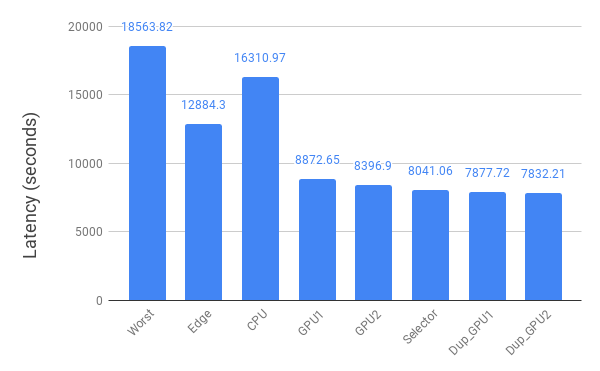
\includegraphics[scale=0.42]{latency.png}
%\caption{The Total Latency of the worst scenario, single runtimes, selector
%and duplicators. } \label{fig:latency} \end{figure}
%
%We next analyze the duplicator of edge cloud versus gpu2. According to the MDE
%metric, gpu2 runtime has more variable deployment and processing time compared
%to gpu1 runtime, which possibly leads to a lower success rate of selection.
%The analytics of the data proves this assumption that STOIC only makes right
%selection between edge cloud and gpu2 runtime by 94.8\% of times, 1.9\% lower
%than being with gpu1 runtime. However, as depicted in the
%Figure~\ref{fig:latency}, the total latency of single gpu2 runtime is shorter
%than the total latency for single gpu1 runtime. We argue that even though
%STOIC make slightly more mistakes in this mode, the duplicator of gpu2 forms a
%faster and more efficient dispatching system. Demonstrated in the
%Table~\ref{tab:comparison}, duplicator of gpu2 runtime achieves the lowest
%average latency (50.86 seconds) and highest speedup (2.37x). We plan to
%investigate runtimes with more GPUs and the trade-off between the
%predictability and efficiency of system as future work.

\iffalse
Table~\ref{tab:success} summarizes the possible success failure cases for the
Duplicator.
\begin{table}[t] 
\centering
\captionsetup{justification=centering}
\scriptsize
\resizebox{\columnwidth}{!}{
\begin{tabular}{|c|c|c|c|} 
\hline
\textbf{\makecell{Predicted GPU \\Lower Latency}} & \textbf{Switch to GPU} & \textbf{\makecell{Actual GPU \\Lower Latency} } & \textbf{Case Label}\\
\hline
Yes & Yes & Yes & Success \\
\hline
Yes & Yes & No & Success \\
\hline
Yes & No & Yes & \textbf{Failure} \\
\hline
Yes & No & No & Success \\
\hline
No & Yes & Yes & Success\\
\hline
No & Yes & No & Success \\
\hline
No & No & Yes & \textbf{Failure} \\
\hline
No & No & No & Success \\
\hline
\end{tabular}
}
\caption{
Duplicator success/failure cases for STOIC.}
\label{tab:success}
\end{table}

\begin{algorithm}[]
\caption{Duplicator Success Rate Heuristic}
\label{algo:optimizer}
\SetAlgoLined
\KwData{Executions on Edge and GPUx runtime}
\KwResult{Runtime Selection Labels}
\For{Executions on Edge and GPUx}{
 \eIf{Predicted GPUx $T_s$ $<$ Predicted Edge $T_s$}{
    \eIf{Predicted Edge $T_s$ - (Actual GPUs $T_t$ + Actual GPUs $T_d$)) $\ge$ Predicted GPUx $T_s$}{
    \eIf{Actual GPUx $T_s$ $<$ Actual Edge $T_s$}{SUCCESS}{SUCCESS}
 }{
    \eIf{Actual GPUx $T_s$ $<$ Actual Edge $T_s$}{FAILURE}{SUCCESS}}}
 {
 \eIf{Predicted Edge $T_s$ - (Actual GPUs $T_t$ + Actual GPUs $T_d$)) $\ge$ Predicted GPUx $T_s$}{
    \eIf{Actual GPUx $T_s$ $<$ Actual Edge $T_s$}{SUCCESS}{SUCCESS}
 }{
    \eIf{Acutal GPUx $T_s$ $<$ Actual Edge $T_s$}{FAILURE}{SUCCESS}}
 }
}
\end{algorithm}
\fi
